% Created by tikzDevice version 0.12 on 2019-10-11 15:46:25
% !TEX encoding = UTF-8 Unicode
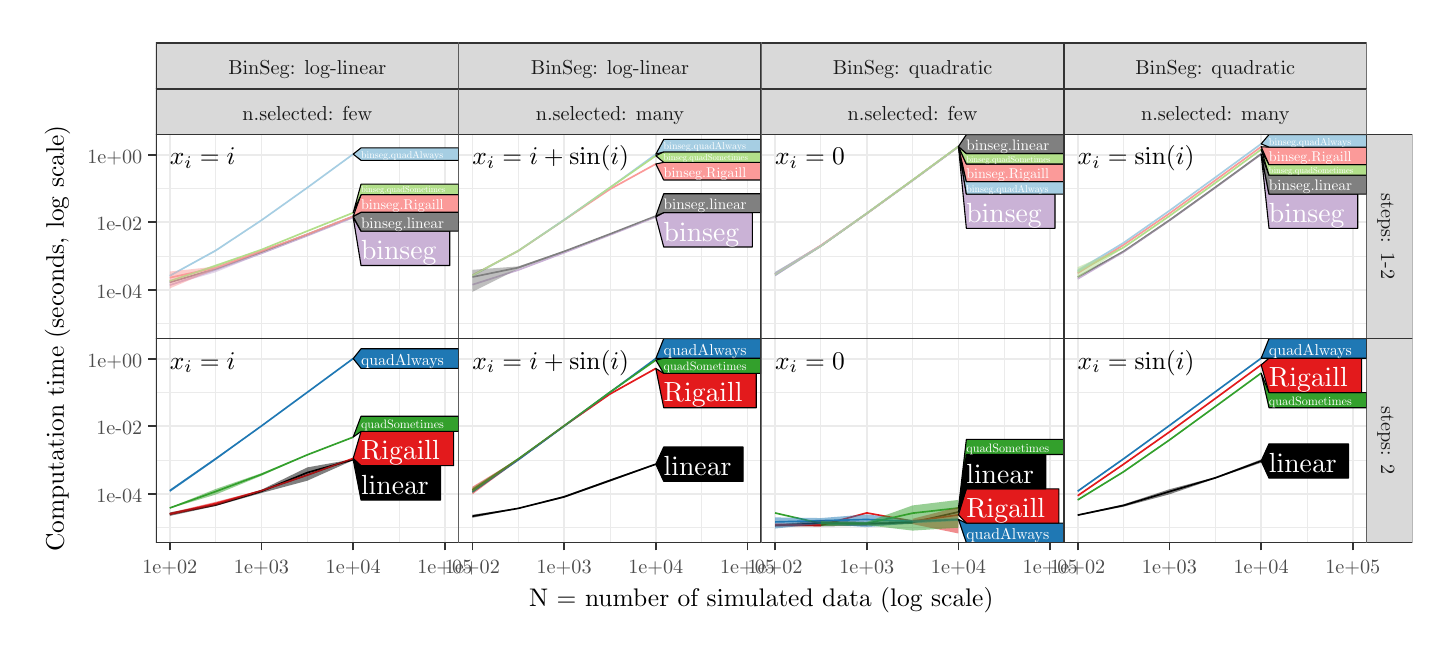
\begin{tikzpicture}[x=1pt,y=1pt]
\definecolor{fillColor}{RGB}{255,255,255}
\path[use as bounding box,fill=fillColor,fill opacity=0.00] (0,0) rectangle (505.89,216.81);
\begin{scope}
\path[clip] (  0.00,  0.00) rectangle (505.89,216.81);
\definecolor{drawColor}{RGB}{255,255,255}
\definecolor{fillColor}{RGB}{255,255,255}

\path[draw=drawColor,line width= 0.6pt,line join=round,line cap=round,fill=fillColor] (  0.00,  0.00) rectangle (505.89,216.81);
\end{scope}
\begin{scope}
\path[clip] ( 46.36,104.43) rectangle (155.73,178.17);
\definecolor{fillColor}{RGB}{255,255,255}

\path[fill=fillColor] ( 46.36,104.43) rectangle (155.73,178.17);
\definecolor{drawColor}{gray}{0.92}

\path[draw=drawColor,line width= 0.3pt,line join=round] ( 46.36,109.94) --
	(155.73,109.94);

\path[draw=drawColor,line width= 0.3pt,line join=round] ( 46.36,134.31) --
	(155.73,134.31);

\path[draw=drawColor,line width= 0.3pt,line join=round] ( 46.36,158.68) --
	(155.73,158.68);

\path[draw=drawColor,line width= 0.3pt,line join=round] ( 67.91,104.43) --
	( 67.91,178.17);

\path[draw=drawColor,line width= 0.3pt,line join=round] (101.05,104.43) --
	(101.05,178.17);

\path[draw=drawColor,line width= 0.3pt,line join=round] (134.19,104.43) --
	(134.19,178.17);

\path[draw=drawColor,line width= 0.6pt,line join=round] ( 46.36,122.13) --
	(155.73,122.13);

\path[draw=drawColor,line width= 0.6pt,line join=round] ( 46.36,146.50) --
	(155.73,146.50);

\path[draw=drawColor,line width= 0.6pt,line join=round] ( 46.36,170.87) --
	(155.73,170.87);

\path[draw=drawColor,line width= 0.6pt,line join=round] ( 51.34,104.43) --
	( 51.34,178.17);

\path[draw=drawColor,line width= 0.6pt,line join=round] ( 84.48,104.43) --
	( 84.48,178.17);

\path[draw=drawColor,line width= 0.6pt,line join=round] (117.62,104.43) --
	(117.62,178.17);

\path[draw=drawColor,line width= 0.6pt,line join=round] (150.76,104.43) --
	(150.76,178.17);
\definecolor{drawColor}{RGB}{0,0,0}

\node[text=drawColor,anchor=base west,inner sep=0pt, outer sep=0pt, scale=  0.92] at ( 51.34,167.21) {$x_i = i$};
\definecolor{drawColor}{RGB}{202,178,214}

\path[draw=drawColor,line width= 0.6pt,line join=round] ( 51.34,123.75) --
	( 67.91,129.32) --
	( 84.48,135.26) --
	(101.05,141.64) --
	(117.62,148.23);
\definecolor{drawColor}{gray}{0.50}

\path[draw=drawColor,line width= 0.6pt,line join=round] ( 51.34,124.78) --
	( 67.91,129.63) --
	( 84.48,135.78) --
	(101.05,142.11) --
	(117.62,148.59);
\definecolor{drawColor}{RGB}{251,154,153}

\path[draw=drawColor,line width= 0.6pt,line join=round] ( 51.34,126.47) --
	( 67.91,130.03) --
	( 84.48,136.04) --
	(101.05,142.14) --
	(117.62,148.64);
\definecolor{drawColor}{RGB}{166,206,227}

\path[draw=drawColor,line width= 0.6pt,line join=round] ( 51.34,127.16) --
	( 67.91,136.26) --
	( 84.48,147.22) --
	(101.05,159.00) --
	(117.62,171.11);
\definecolor{drawColor}{RGB}{178,223,138}

\path[draw=drawColor,line width= 0.6pt,line join=round] ( 51.34,125.26) --
	( 67.91,130.77) --
	( 84.48,136.59) --
	(101.05,143.32) --
	(117.62,149.93);
\definecolor{fillColor}{RGB}{202,178,214}

\path[fill=fillColor,fill opacity=0.50] ( 51.34,123.88) --
	( 67.91,130.09) --
	( 84.48,135.41) --
	(101.05,141.68) --
	(117.62,148.42) --
	(117.62,148.04) --
	(101.05,141.60) --
	( 84.48,135.10) --
	( 67.91,128.41) --
	( 51.34,123.62) --
	cycle;
\definecolor{fillColor}{RGB}{127,127,127}

\path[fill=fillColor,fill opacity=0.50] ( 51.34,124.93) --
	( 67.91,129.70) --
	( 84.48,135.99) --
	(101.05,142.16) --
	(117.62,148.62) --
	(117.62,148.57) --
	(101.05,142.06) --
	( 84.48,135.55) --
	( 67.91,129.55) --
	( 51.34,124.63) --
	cycle;
\definecolor{fillColor}{RGB}{251,154,153}

\path[fill=fillColor,fill opacity=0.50] ( 51.34,128.69) --
	( 67.91,130.47) --
	( 84.48,136.45) --
	(101.05,142.17) --
	(117.62,148.69) --
	(117.62,148.58) --
	(101.05,142.11) --
	( 84.48,135.58) --
	( 67.91,129.56) --
	( 51.34,122.59) --
	cycle;
\definecolor{fillColor}{RGB}{166,206,227}

\path[fill=fillColor,fill opacity=0.50] ( 51.34,127.30) --
	( 67.91,136.53) --
	( 84.48,147.25) --
	(101.05,159.01) --
	(117.62,171.21) --
	(117.62,171.01) --
	(101.05,159.00) --
	( 84.48,147.19) --
	( 67.91,135.97) --
	( 51.34,127.03) --
	cycle;
\definecolor{fillColor}{RGB}{178,223,138}

\path[fill=fillColor,fill opacity=0.50] ( 51.34,125.41) --
	( 67.91,131.22) --
	( 84.48,136.65) --
	(101.05,143.36) --
	(117.62,150.12) --
	(117.62,149.72) --
	(101.05,143.29) --
	( 84.48,136.52) --
	( 67.91,130.29) --
	( 51.34,125.11) --
	cycle;
\end{scope}
\begin{scope}
\path[clip] ( 46.36,104.43) rectangle (155.73,178.17);
\definecolor{drawColor}{RGB}{0,0,0}
\definecolor{fillColor}{RGB}{202,178,214}

\path[draw=drawColor,line width= 0.4pt,line join=round,line cap=round,fill=fillColor] (117.62,148.23) --
	(120.46,143.27) --
	(152.51,143.27) --
	(152.51,130.87) --
	(120.46,130.87) --
	cycle;
\definecolor{fillColor}{gray}{0.50}

\path[draw=drawColor,line width= 0.4pt,line join=round,line cap=round,fill=fillColor] (117.62,148.59) --
	(120.46,150.10) --
	(155.72,150.10) --
	(155.72,143.27) --
	(120.46,143.27) --
	cycle;
\definecolor{fillColor}{RGB}{251,154,153}

\path[draw=drawColor,line width= 0.4pt,line join=round,line cap=round,fill=fillColor] (117.62,148.64) --
	(120.46,156.46) --
	(155.73,156.46) --
	(155.73,150.10) --
	(120.46,150.10) --
	cycle;
\definecolor{fillColor}{RGB}{178,223,138}

\path[draw=drawColor,line width= 0.4pt,line join=round,line cap=round,fill=fillColor] (117.62,149.93) --
	(120.46,160.25) --
	(155.73,160.25) --
	(155.73,156.46) --
	(120.46,156.46) --
	cycle;
\definecolor{fillColor}{RGB}{166,206,227}

\path[draw=drawColor,line width= 0.4pt,line join=round,line cap=round,fill=fillColor] (117.62,171.11) --
	(120.46,173.36) --
	(155.73,173.36) --
	(155.73,168.86) --
	(120.46,168.86) --
	cycle;
\definecolor{drawColor}{RGB}{255,255,255}

\node[text=drawColor,anchor=base west,inner sep=0pt, outer sep=0pt, scale=  1.00] at (120.46,132.94) {binseg};

\node[text=drawColor,anchor=base west,inner sep=0pt, outer sep=0pt, scale=  0.55] at (120.46,144.41) {binseg.linear};

\node[text=drawColor,anchor=base west,inner sep=0pt, outer sep=0pt, scale=  0.51] at (120.46,151.16) {binseg.Rigaill};

\node[text=drawColor,anchor=base west,inner sep=0pt, outer sep=0pt, scale=  0.31] at (120.46,157.09) {binseg.quadSometimes};

\node[text=drawColor,anchor=base west,inner sep=0pt, outer sep=0pt, scale=  0.36] at (120.46,169.61) {binseg.quadAlways};
\definecolor{drawColor}{gray}{0.20}

\path[draw=drawColor,line width= 0.6pt,line join=round,line cap=round] ( 46.36,104.43) rectangle (155.73,178.17);
\end{scope}
\begin{scope}
\path[clip] ( 46.36, 30.69) rectangle (155.73,104.43);
\definecolor{fillColor}{RGB}{255,255,255}

\path[fill=fillColor] ( 46.36, 30.69) rectangle (155.73,104.43);
\definecolor{drawColor}{gray}{0.92}

\path[draw=drawColor,line width= 0.3pt,line join=round] ( 46.36, 36.20) --
	(155.73, 36.20);

\path[draw=drawColor,line width= 0.3pt,line join=round] ( 46.36, 60.57) --
	(155.73, 60.57);

\path[draw=drawColor,line width= 0.3pt,line join=round] ( 46.36, 84.94) --
	(155.73, 84.94);

\path[draw=drawColor,line width= 0.3pt,line join=round] ( 67.91, 30.69) --
	( 67.91,104.43);

\path[draw=drawColor,line width= 0.3pt,line join=round] (101.05, 30.69) --
	(101.05,104.43);

\path[draw=drawColor,line width= 0.3pt,line join=round] (134.19, 30.69) --
	(134.19,104.43);

\path[draw=drawColor,line width= 0.6pt,line join=round] ( 46.36, 48.39) --
	(155.73, 48.39);

\path[draw=drawColor,line width= 0.6pt,line join=round] ( 46.36, 72.76) --
	(155.73, 72.76);

\path[draw=drawColor,line width= 0.6pt,line join=round] ( 46.36, 97.13) --
	(155.73, 97.13);

\path[draw=drawColor,line width= 0.6pt,line join=round] ( 51.34, 30.69) --
	( 51.34,104.43);

\path[draw=drawColor,line width= 0.6pt,line join=round] ( 84.48, 30.69) --
	( 84.48,104.43);

\path[draw=drawColor,line width= 0.6pt,line join=round] (117.62, 30.69) --
	(117.62,104.43);

\path[draw=drawColor,line width= 0.6pt,line join=round] (150.76, 30.69) --
	(150.76,104.43);
\definecolor{drawColor}{RGB}{0,0,0}

\node[text=drawColor,anchor=base west,inner sep=0pt, outer sep=0pt, scale=  0.92] at ( 51.34, 93.47) {$x_i = i$};

\path[draw=drawColor,line width= 0.6pt,line join=round] ( 51.34, 41.05) --
	( 67.91, 44.34) --
	( 84.48, 49.28) --
	(101.05, 56.04) --
	(117.62, 60.70);
\definecolor{drawColor}{RGB}{227,26,28}

\path[draw=drawColor,line width= 0.6pt,line join=round] ( 51.34, 41.11) --
	( 67.91, 44.85) --
	( 84.48, 49.50) --
	(101.05, 55.14) --
	(117.62, 61.16);
\definecolor{drawColor}{RGB}{31,120,180}

\path[draw=drawColor,line width= 0.6pt,line join=round] ( 51.34, 49.45) --
	( 67.91, 60.99) --
	( 84.48, 72.89) --
	(101.05, 85.06) --
	(117.62, 97.25);
\definecolor{drawColor}{RGB}{51,160,44}

\path[draw=drawColor,line width= 0.6pt,line join=round] ( 51.34, 43.25) --
	( 67.91, 49.19) --
	( 84.48, 55.38) --
	(101.05, 62.46) --
	(117.62, 68.84);
\definecolor{fillColor}{RGB}{0,0,0}

\path[fill=fillColor,fill opacity=0.50] ( 51.34, 41.64) --
	( 67.91, 44.70) --
	( 84.48, 49.84) --
	(101.05, 57.91) --
	(117.62, 60.87) --
	(117.62, 60.52) --
	(101.05, 53.11) --
	( 84.48, 48.66) --
	( 67.91, 43.96) --
	( 51.34, 40.37) --
	cycle;
\definecolor{fillColor}{RGB}{227,26,28}

\path[fill=fillColor,fill opacity=0.50] ( 51.34, 41.52) --
	( 67.91, 45.45) --
	( 84.48, 49.73) --
	(101.05, 55.39) --
	(117.62, 61.24) --
	(117.62, 61.09) --
	(101.05, 54.87) --
	( 84.48, 49.26) --
	( 67.91, 44.16) --
	( 51.34, 40.66) --
	cycle;
\definecolor{fillColor}{RGB}{31,120,180}

\path[fill=fillColor,fill opacity=0.50] ( 51.34, 49.88) --
	( 67.91, 61.36) --
	( 84.48, 72.90) --
	(101.05, 85.07) --
	(117.62, 97.26) --
	(117.62, 97.25) --
	(101.05, 85.05) --
	( 84.48, 72.88) --
	( 67.91, 60.59) --
	( 51.34, 48.97) --
	cycle;
\definecolor{fillColor}{RGB}{51,160,44}

\path[fill=fillColor,fill opacity=0.50] ( 51.34, 43.39) --
	( 67.91, 50.11) --
	( 84.48, 55.82) --
	(101.05, 62.58) --
	(117.62, 68.96) --
	(117.62, 68.72) --
	(101.05, 62.34) --
	( 84.48, 54.90) --
	( 67.91, 48.08) --
	( 51.34, 43.10) --
	cycle;
\end{scope}
\begin{scope}
\path[clip] ( 46.36, 30.69) rectangle (155.73,104.43);
\definecolor{drawColor}{RGB}{0,0,0}
\definecolor{fillColor}{RGB}{0,0,0}

\path[draw=drawColor,line width= 0.4pt,line join=round,line cap=round,fill=fillColor] (117.62, 60.70) --
	(120.46, 58.53) --
	(149.18, 58.53) --
	(149.18, 46.13) --
	(120.46, 46.13) --
	cycle;
\definecolor{fillColor}{RGB}{227,26,28}

\path[draw=drawColor,line width= 0.4pt,line join=round,line cap=round,fill=fillColor] (117.62, 61.16) --
	(120.46, 70.92) --
	(153.91, 70.92) --
	(153.91, 58.53) --
	(120.46, 58.53) --
	cycle;
\definecolor{fillColor}{RGB}{51,160,44}

\path[draw=drawColor,line width= 0.4pt,line join=round,line cap=round,fill=fillColor] (117.62, 68.84) --
	(120.46, 76.39) --
	(155.73, 76.39) --
	(155.73, 70.92) --
	(120.46, 70.92) --
	cycle;
\definecolor{fillColor}{RGB}{31,120,180}

\path[draw=drawColor,line width= 0.4pt,line join=round,line cap=round,fill=fillColor] (117.62, 97.25) --
	(120.46,100.80) --
	(155.73,100.80) --
	(155.73, 93.71) --
	(120.46, 93.71) --
	cycle;
\definecolor{drawColor}{RGB}{255,255,255}

\node[text=drawColor,anchor=base west,inner sep=0pt, outer sep=0pt, scale=  1.00] at (120.46, 48.20) {linear};

\node[text=drawColor,anchor=base west,inner sep=0pt, outer sep=0pt, scale=  1.00] at (120.46, 60.59) {Rigaill};

\node[text=drawColor,anchor=base west,inner sep=0pt, outer sep=0pt, scale=  0.44] at (120.46, 71.83) {quadSometimes};

\node[text=drawColor,anchor=base west,inner sep=0pt, outer sep=0pt, scale=  0.57] at (120.46, 94.89) {quadAlways};
\definecolor{drawColor}{gray}{0.20}

\path[draw=drawColor,line width= 0.6pt,line join=round,line cap=round] ( 46.36, 30.69) rectangle (155.73,104.43);
\end{scope}
\begin{scope}
\path[clip] (155.73,104.43) rectangle (265.09,178.17);
\definecolor{fillColor}{RGB}{255,255,255}

\path[fill=fillColor] (155.73,104.43) rectangle (265.09,178.17);
\definecolor{drawColor}{gray}{0.92}

\path[draw=drawColor,line width= 0.3pt,line join=round] (155.73,109.94) --
	(265.09,109.94);

\path[draw=drawColor,line width= 0.3pt,line join=round] (155.73,134.31) --
	(265.09,134.31);

\path[draw=drawColor,line width= 0.3pt,line join=round] (155.73,158.68) --
	(265.09,158.68);

\path[draw=drawColor,line width= 0.3pt,line join=round] (177.27,104.43) --
	(177.27,178.17);

\path[draw=drawColor,line width= 0.3pt,line join=round] (210.41,104.43) --
	(210.41,178.17);

\path[draw=drawColor,line width= 0.3pt,line join=round] (243.55,104.43) --
	(243.55,178.17);

\path[draw=drawColor,line width= 0.6pt,line join=round] (155.73,122.13) --
	(265.09,122.13);

\path[draw=drawColor,line width= 0.6pt,line join=round] (155.73,146.50) --
	(265.09,146.50);

\path[draw=drawColor,line width= 0.6pt,line join=round] (155.73,170.87) --
	(265.09,170.87);

\path[draw=drawColor,line width= 0.6pt,line join=round] (160.70,104.43) --
	(160.70,178.17);

\path[draw=drawColor,line width= 0.6pt,line join=round] (193.84,104.43) --
	(193.84,178.17);

\path[draw=drawColor,line width= 0.6pt,line join=round] (226.98,104.43) --
	(226.98,178.17);

\path[draw=drawColor,line width= 0.6pt,line join=round] (260.12,104.43) --
	(260.12,178.17);
\definecolor{drawColor}{RGB}{0,0,0}

\node[text=drawColor,anchor=base west,inner sep=0pt, outer sep=0pt, scale=  0.92] at (160.70,167.21) {$x_i = i+\sin(i)$};
\definecolor{drawColor}{RGB}{202,178,214}

\path[draw=drawColor,line width= 0.6pt,line join=round] (160.70,123.93) --
	(177.27,129.24) --
	(193.84,135.49) --
	(210.41,141.92) --
	(226.98,148.42);
\definecolor{drawColor}{gray}{0.50}

\path[draw=drawColor,line width= 0.6pt,line join=round] (160.70,126.71) --
	(177.27,130.11) --
	(193.84,135.95) --
	(210.41,142.25) --
	(226.98,148.73);
\definecolor{drawColor}{RGB}{251,154,153}

\path[draw=drawColor,line width= 0.6pt,line join=round] (160.70,127.31) --
	(177.27,136.13) --
	(193.84,147.29) --
	(210.41,158.44) --
	(226.98,167.56);
\definecolor{drawColor}{RGB}{166,206,227}

\path[draw=drawColor,line width= 0.6pt,line join=round] (160.70,127.21) --
	(177.27,136.16) --
	(193.84,147.36) --
	(210.41,159.00) --
	(226.98,171.07);
\definecolor{drawColor}{RGB}{178,223,138}

\path[draw=drawColor,line width= 0.6pt,line join=round] (160.70,127.27) --
	(177.27,136.18) --
	(193.84,147.30) --
	(210.41,159.03) --
	(226.98,170.52);
\definecolor{fillColor}{RGB}{202,178,214}

\path[fill=fillColor,fill opacity=0.50] (160.70,123.97) --
	(177.27,129.32) --
	(193.84,135.58) --
	(210.41,141.94) --
	(226.98,148.58) --
	(226.98,148.26) --
	(210.41,141.91) --
	(193.84,135.39) --
	(177.27,129.16) --
	(160.70,123.89) --
	cycle;
\definecolor{fillColor}{RGB}{127,127,127}

\path[fill=fillColor,fill opacity=0.50] (160.70,129.31) --
	(177.27,130.55) --
	(193.84,136.13) --
	(210.41,142.29) --
	(226.98,148.84) --
	(226.98,148.63) --
	(210.41,142.21) --
	(193.84,135.76) --
	(177.27,129.64) --
	(160.70,121.36) --
	cycle;
\definecolor{fillColor}{RGB}{251,154,153}

\path[fill=fillColor,fill opacity=0.50] (160.70,127.44) --
	(177.27,136.22) --
	(193.84,147.37) --
	(210.41,158.53) --
	(226.98,167.56) --
	(226.98,167.55) --
	(210.41,158.34) --
	(193.84,147.20) --
	(177.27,136.04) --
	(160.70,127.17) --
	cycle;
\definecolor{fillColor}{RGB}{166,206,227}

\path[fill=fillColor,fill opacity=0.50] (160.70,127.30) --
	(177.27,136.23) --
	(193.84,147.68) --
	(210.41,159.00) --
	(226.98,171.07) --
	(226.98,171.06) --
	(210.41,159.00) --
	(193.84,147.03) --
	(177.27,136.09) --
	(160.70,127.12) --
	cycle;
\definecolor{fillColor}{RGB}{178,223,138}

\path[fill=fillColor,fill opacity=0.50] (160.70,127.61) --
	(177.27,136.24) --
	(193.84,147.34) --
	(210.41,159.04) --
	(226.98,170.53) --
	(226.98,170.51) --
	(210.41,159.02) --
	(193.84,147.27) --
	(177.27,136.12) --
	(160.70,126.91) --
	cycle;
\end{scope}
\begin{scope}
\path[clip] (155.73,104.43) rectangle (265.09,178.17);
\definecolor{drawColor}{RGB}{0,0,0}
\definecolor{fillColor}{RGB}{202,178,214}

\path[draw=drawColor,line width= 0.4pt,line join=round,line cap=round,fill=fillColor] (226.98,148.42) --
	(229.83,149.97) --
	(261.87,149.97) --
	(261.87,137.57) --
	(229.83,137.57) --
	cycle;
\definecolor{fillColor}{gray}{0.50}

\path[draw=drawColor,line width= 0.4pt,line join=round,line cap=round,fill=fillColor] (226.98,148.73) --
	(229.83,156.80) --
	(265.09,156.80) --
	(265.09,149.97) --
	(229.83,149.97) --
	cycle;
\definecolor{fillColor}{RGB}{251,154,153}

\path[draw=drawColor,line width= 0.4pt,line join=round,line cap=round,fill=fillColor] (226.98,167.56) --
	(229.83,168.13) --
	(265.09,168.13) --
	(265.09,161.77) --
	(229.83,161.77) --
	cycle;
\definecolor{fillColor}{RGB}{178,223,138}

\path[draw=drawColor,line width= 0.4pt,line join=round,line cap=round,fill=fillColor] (226.98,170.52) --
	(229.83,171.92) --
	(265.09,171.92) --
	(265.09,168.13) --
	(229.83,168.13) --
	cycle;
\definecolor{fillColor}{RGB}{166,206,227}

\path[draw=drawColor,line width= 0.4pt,line join=round,line cap=round,fill=fillColor] (226.98,171.07) --
	(229.83,176.43) --
	(265.09,176.43) --
	(265.09,171.92) --
	(229.83,171.92) --
	cycle;
\definecolor{drawColor}{RGB}{255,255,255}

\node[text=drawColor,anchor=base west,inner sep=0pt, outer sep=0pt, scale=  1.00] at (229.83,139.64) {binseg};

\node[text=drawColor,anchor=base west,inner sep=0pt, outer sep=0pt, scale=  0.55] at (229.83,151.11) {binseg.linear};

\node[text=drawColor,anchor=base west,inner sep=0pt, outer sep=0pt, scale=  0.51] at (229.83,162.83) {binseg.Rigaill};

\node[text=drawColor,anchor=base west,inner sep=0pt, outer sep=0pt, scale=  0.31] at (229.83,168.76) {binseg.quadSometimes};

\node[text=drawColor,anchor=base west,inner sep=0pt, outer sep=0pt, scale=  0.36] at (229.83,172.67) {binseg.quadAlways};
\definecolor{drawColor}{gray}{0.20}

\path[draw=drawColor,line width= 0.6pt,line join=round,line cap=round] (155.73,104.43) rectangle (265.09,178.17);
\end{scope}
\begin{scope}
\path[clip] (155.73, 30.69) rectangle (265.09,104.43);
\definecolor{fillColor}{RGB}{255,255,255}

\path[fill=fillColor] (155.73, 30.69) rectangle (265.09,104.43);
\definecolor{drawColor}{gray}{0.92}

\path[draw=drawColor,line width= 0.3pt,line join=round] (155.73, 36.20) --
	(265.09, 36.20);

\path[draw=drawColor,line width= 0.3pt,line join=round] (155.73, 60.57) --
	(265.09, 60.57);

\path[draw=drawColor,line width= 0.3pt,line join=round] (155.73, 84.94) --
	(265.09, 84.94);

\path[draw=drawColor,line width= 0.3pt,line join=round] (177.27, 30.69) --
	(177.27,104.43);

\path[draw=drawColor,line width= 0.3pt,line join=round] (210.41, 30.69) --
	(210.41,104.43);

\path[draw=drawColor,line width= 0.3pt,line join=round] (243.55, 30.69) --
	(243.55,104.43);

\path[draw=drawColor,line width= 0.6pt,line join=round] (155.73, 48.39) --
	(265.09, 48.39);

\path[draw=drawColor,line width= 0.6pt,line join=round] (155.73, 72.76) --
	(265.09, 72.76);

\path[draw=drawColor,line width= 0.6pt,line join=round] (155.73, 97.13) --
	(265.09, 97.13);

\path[draw=drawColor,line width= 0.6pt,line join=round] (160.70, 30.69) --
	(160.70,104.43);

\path[draw=drawColor,line width= 0.6pt,line join=round] (193.84, 30.69) --
	(193.84,104.43);

\path[draw=drawColor,line width= 0.6pt,line join=round] (226.98, 30.69) --
	(226.98,104.43);

\path[draw=drawColor,line width= 0.6pt,line join=round] (260.12, 30.69) --
	(260.12,104.43);
\definecolor{drawColor}{RGB}{0,0,0}

\node[text=drawColor,anchor=base west,inner sep=0pt, outer sep=0pt, scale=  0.92] at (160.70, 93.47) {$x_i = i+\sin(i)$};

\path[draw=drawColor,line width= 0.6pt,line join=round] (160.70, 40.28) --
	(177.27, 43.10) --
	(193.84, 47.27) --
	(210.41, 53.19) --
	(226.98, 59.08);
\definecolor{drawColor}{RGB}{227,26,28}

\path[draw=drawColor,line width= 0.6pt,line join=round] (160.70, 49.73) --
	(177.27, 60.79) --
	(193.84, 72.91) --
	(210.41, 84.42) --
	(226.98, 93.67);
\definecolor{drawColor}{RGB}{31,120,180}

\path[draw=drawColor,line width= 0.6pt,line join=round] (160.70, 49.04) --
	(177.27, 60.64) --
	(193.84, 72.85) --
	(210.41, 85.04) --
	(226.98, 97.25);
\definecolor{drawColor}{RGB}{51,160,44}

\path[draw=drawColor,line width= 0.6pt,line join=round] (160.70, 49.65) --
	(177.27, 60.97) --
	(193.84, 72.93) --
	(210.41, 85.09) --
	(226.98, 96.70);
\definecolor{fillColor}{RGB}{0,0,0}

\path[fill=fillColor,fill opacity=0.50] (160.70, 40.81) --
	(177.27, 43.22) --
	(193.84, 47.59) --
	(210.41, 53.56) --
	(226.98, 59.27) --
	(226.98, 58.89) --
	(210.41, 52.78) --
	(193.84, 46.93) --
	(177.27, 42.97) --
	(160.70, 39.70) --
	cycle;
\definecolor{fillColor}{RGB}{227,26,28}

\path[fill=fillColor,fill opacity=0.50] (160.70, 50.93) --
	(177.27, 61.02) --
	(193.84, 73.00) --
	(210.41, 84.52) --
	(226.98, 93.69) --
	(226.98, 93.65) --
	(210.41, 84.31) --
	(193.84, 72.82) --
	(177.27, 60.54) --
	(160.70, 48.16) --
	cycle;
\definecolor{fillColor}{RGB}{31,120,180}

\path[fill=fillColor,fill opacity=0.50] (160.70, 49.24) --
	(177.27, 60.77) --
	(193.84, 72.89) --
	(210.41, 85.05) --
	(226.98, 97.26) --
	(226.98, 97.25) --
	(210.41, 85.04) --
	(193.84, 72.82) --
	(177.27, 60.50) --
	(160.70, 48.82) --
	cycle;
\definecolor{fillColor}{RGB}{51,160,44}

\path[fill=fillColor,fill opacity=0.50] (160.70, 50.44) --
	(177.27, 61.27) --
	(193.84, 72.96) --
	(210.41, 85.11) --
	(226.98, 96.70) --
	(226.98, 96.69) --
	(210.41, 85.07) --
	(193.84, 72.91) --
	(177.27, 60.65) --
	(160.70, 48.72) --
	cycle;
\end{scope}
\begin{scope}
\path[clip] (155.73, 30.69) rectangle (265.09,104.43);
\definecolor{drawColor}{RGB}{0,0,0}
\definecolor{fillColor}{RGB}{0,0,0}

\path[draw=drawColor,line width= 0.4pt,line join=round,line cap=round,fill=fillColor] (226.98, 59.08) --
	(229.83, 65.28) --
	(258.54, 65.28) --
	(258.54, 52.89) --
	(229.83, 52.89) --
	cycle;
\definecolor{fillColor}{RGB}{227,26,28}

\path[draw=drawColor,line width= 0.4pt,line join=round,line cap=round,fill=fillColor] (226.98, 93.67) --
	(229.83, 91.88) --
	(263.27, 91.88) --
	(263.27, 79.48) --
	(229.83, 79.48) --
	cycle;
\definecolor{fillColor}{RGB}{51,160,44}

\path[draw=drawColor,line width= 0.4pt,line join=round,line cap=round,fill=fillColor] (226.98, 96.70) --
	(229.83, 97.34) --
	(265.09, 97.34) --
	(265.09, 91.88) --
	(229.83, 91.88) --
	cycle;
\definecolor{fillColor}{RGB}{31,120,180}

\path[draw=drawColor,line width= 0.4pt,line join=round,line cap=round,fill=fillColor] (226.98, 97.25) --
	(229.83,104.43) --
	(265.09,104.43) --
	(265.09, 97.34) --
	(229.83, 97.34) --
	cycle;
\definecolor{drawColor}{RGB}{255,255,255}

\node[text=drawColor,anchor=base west,inner sep=0pt, outer sep=0pt, scale=  1.00] at (229.83, 54.95) {linear};

\node[text=drawColor,anchor=base west,inner sep=0pt, outer sep=0pt, scale=  1.00] at (229.83, 81.55) {Rigaill};

\node[text=drawColor,anchor=base west,inner sep=0pt, outer sep=0pt, scale=  0.44] at (229.83, 92.79) {quadSometimes};

\node[text=drawColor,anchor=base west,inner sep=0pt, outer sep=0pt, scale=  0.57] at (229.83, 98.52) {quadAlways};
\definecolor{drawColor}{gray}{0.20}

\path[draw=drawColor,line width= 0.6pt,line join=round,line cap=round] (155.73, 30.69) rectangle (265.09,104.43);
\end{scope}
\begin{scope}
\path[clip] (265.09,104.43) rectangle (374.46,178.17);
\definecolor{fillColor}{RGB}{255,255,255}

\path[fill=fillColor] (265.09,104.43) rectangle (374.46,178.17);
\definecolor{drawColor}{gray}{0.92}

\path[draw=drawColor,line width= 0.3pt,line join=round] (265.09,109.94) --
	(374.46,109.94);

\path[draw=drawColor,line width= 0.3pt,line join=round] (265.09,134.31) --
	(374.46,134.31);

\path[draw=drawColor,line width= 0.3pt,line join=round] (265.09,158.68) --
	(374.46,158.68);

\path[draw=drawColor,line width= 0.3pt,line join=round] (286.63,104.43) --
	(286.63,178.17);

\path[draw=drawColor,line width= 0.3pt,line join=round] (319.77,104.43) --
	(319.77,178.17);

\path[draw=drawColor,line width= 0.3pt,line join=round] (352.91,104.43) --
	(352.91,178.17);

\path[draw=drawColor,line width= 0.6pt,line join=round] (265.09,122.13) --
	(374.46,122.13);

\path[draw=drawColor,line width= 0.6pt,line join=round] (265.09,146.50) --
	(374.46,146.50);

\path[draw=drawColor,line width= 0.6pt,line join=round] (265.09,170.87) --
	(374.46,170.87);

\path[draw=drawColor,line width= 0.6pt,line join=round] (270.06,104.43) --
	(270.06,178.17);

\path[draw=drawColor,line width= 0.6pt,line join=round] (303.20,104.43) --
	(303.20,178.17);

\path[draw=drawColor,line width= 0.6pt,line join=round] (336.34,104.43) --
	(336.34,178.17);

\path[draw=drawColor,line width= 0.6pt,line join=round] (369.48,104.43) --
	(369.48,178.17);
\definecolor{drawColor}{RGB}{0,0,0}

\node[text=drawColor,anchor=base west,inner sep=0pt, outer sep=0pt, scale=  0.92] at (270.06,167.21) {$x_i = 0$};
\definecolor{drawColor}{RGB}{202,178,214}

\path[draw=drawColor,line width= 0.6pt,line join=round] (270.06,127.36) --
	(286.63,137.88) --
	(303.20,149.59) --
	(319.77,161.57) --
	(336.34,173.75);
\definecolor{drawColor}{gray}{0.50}

\path[draw=drawColor,line width= 0.6pt,line join=round] (270.06,127.80) --
	(286.63,137.94) --
	(303.20,149.69) --
	(319.77,161.71) --
	(336.34,173.88);
\definecolor{drawColor}{RGB}{251,154,153}

\path[draw=drawColor,line width= 0.6pt,line join=round] (270.06,127.87) --
	(286.63,138.15) --
	(303.20,149.67) --
	(319.77,161.72) --
	(336.34,173.87);
\definecolor{drawColor}{RGB}{166,206,227}

\path[draw=drawColor,line width= 0.6pt,line join=round] (270.06,127.88) --
	(286.63,138.00) --
	(303.20,149.71) --
	(319.77,161.71) --
	(336.34,173.87);
\definecolor{drawColor}{RGB}{178,223,138}

\path[draw=drawColor,line width= 0.6pt,line join=round] (270.06,127.57) --
	(286.63,137.91) --
	(303.20,149.69) --
	(319.77,161.73) --
	(336.34,173.88);
\definecolor{fillColor}{RGB}{202,178,214}

\path[fill=fillColor,fill opacity=0.50] (270.06,127.78) --
	(286.63,138.08) --
	(303.20,149.69) --
	(319.77,161.59) --
	(336.34,173.80) --
	(336.34,173.69) --
	(319.77,161.55) --
	(303.20,149.48) --
	(286.63,137.67) --
	(270.06,126.90) --
	cycle;
\definecolor{fillColor}{RGB}{127,127,127}

\path[fill=fillColor,fill opacity=0.50] (270.06,128.46) --
	(286.63,137.99) --
	(303.20,149.74) --
	(319.77,161.72) --
	(336.34,173.89) --
	(336.34,173.87) --
	(319.77,161.70) --
	(303.20,149.65) --
	(286.63,137.89) --
	(270.06,127.06) --
	cycle;
\definecolor{fillColor}{RGB}{251,154,153}

\path[fill=fillColor,fill opacity=0.50] (270.06,128.37) --
	(286.63,138.37) --
	(303.20,149.69) --
	(319.77,161.73) --
	(336.34,173.88) --
	(336.34,173.87) --
	(319.77,161.70) --
	(303.20,149.65) --
	(286.63,137.91) --
	(270.06,127.31) --
	cycle;
\definecolor{fillColor}{RGB}{166,206,227}

\path[fill=fillColor,fill opacity=0.50] (270.06,128.57) --
	(286.63,138.28) --
	(303.20,149.75) --
	(319.77,161.72) --
	(336.34,173.88) --
	(336.34,173.87) --
	(319.77,161.71) --
	(303.20,149.67) --
	(286.63,137.72) --
	(270.06,127.08) --
	cycle;
\definecolor{fillColor}{RGB}{178,223,138}

\path[fill=fillColor,fill opacity=0.50] (270.06,127.72) --
	(286.63,138.01) --
	(303.20,149.72) --
	(319.77,161.77) --
	(336.34,173.89) --
	(336.34,173.87) --
	(319.77,161.69) --
	(303.20,149.66) --
	(286.63,137.82) --
	(270.06,127.42) --
	cycle;
\end{scope}
\begin{scope}
\path[clip] (265.09,104.43) rectangle (374.46,178.17);
\definecolor{drawColor}{RGB}{0,0,0}
\definecolor{fillColor}{RGB}{202,178,214}

\path[draw=drawColor,line width= 0.4pt,line join=round,line cap=round,fill=fillColor] (336.34,173.75) --
	(339.19,156.68) --
	(371.23,156.68) --
	(371.23,144.29) --
	(339.19,144.29) --
	cycle;
\definecolor{fillColor}{RGB}{166,206,227}

\path[draw=drawColor,line width= 0.4pt,line join=round,line cap=round,fill=fillColor] (336.34,173.87) --
	(339.19,161.19) --
	(374.45,161.19) --
	(374.45,156.68) --
	(339.19,156.68) --
	cycle;
\definecolor{fillColor}{RGB}{251,154,153}

\path[draw=drawColor,line width= 0.4pt,line join=round,line cap=round,fill=fillColor] (336.34,173.87) --
	(339.19,167.55) --
	(374.46,167.55) --
	(374.46,161.19) --
	(339.19,161.19) --
	cycle;
\definecolor{fillColor}{RGB}{178,223,138}

\path[draw=drawColor,line width= 0.4pt,line join=round,line cap=round,fill=fillColor] (336.34,173.88) --
	(339.19,171.34) --
	(374.45,171.34) --
	(374.45,167.55) --
	(339.19,167.55) --
	cycle;
\definecolor{fillColor}{gray}{0.50}

\path[draw=drawColor,line width= 0.4pt,line join=round,line cap=round,fill=fillColor] (336.34,173.88) --
	(339.19,178.17) --
	(374.45,178.17) --
	(374.45,171.34) --
	(339.19,171.34) --
	cycle;
\definecolor{drawColor}{RGB}{255,255,255}

\node[text=drawColor,anchor=base west,inner sep=0pt, outer sep=0pt, scale=  1.00] at (339.19,146.35) {binseg};

\node[text=drawColor,anchor=base west,inner sep=0pt, outer sep=0pt, scale=  0.36] at (339.19,157.43) {binseg.quadAlways};

\node[text=drawColor,anchor=base west,inner sep=0pt, outer sep=0pt, scale=  0.51] at (339.19,162.25) {binseg.Rigaill};

\node[text=drawColor,anchor=base west,inner sep=0pt, outer sep=0pt, scale=  0.31] at (339.19,168.18) {binseg.quadSometimes};

\node[text=drawColor,anchor=base west,inner sep=0pt, outer sep=0pt, scale=  0.55] at (339.19,172.48) {binseg.linear};
\definecolor{drawColor}{gray}{0.20}

\path[draw=drawColor,line width= 0.6pt,line join=round,line cap=round] (265.09,104.43) rectangle (374.46,178.17);
\end{scope}
\begin{scope}
\path[clip] (265.09, 30.69) rectangle (374.46,104.43);
\definecolor{fillColor}{RGB}{255,255,255}

\path[fill=fillColor] (265.09, 30.69) rectangle (374.46,104.43);
\definecolor{drawColor}{gray}{0.92}

\path[draw=drawColor,line width= 0.3pt,line join=round] (265.09, 36.20) --
	(374.46, 36.20);

\path[draw=drawColor,line width= 0.3pt,line join=round] (265.09, 60.57) --
	(374.46, 60.57);

\path[draw=drawColor,line width= 0.3pt,line join=round] (265.09, 84.94) --
	(374.46, 84.94);

\path[draw=drawColor,line width= 0.3pt,line join=round] (286.63, 30.69) --
	(286.63,104.43);

\path[draw=drawColor,line width= 0.3pt,line join=round] (319.77, 30.69) --
	(319.77,104.43);

\path[draw=drawColor,line width= 0.3pt,line join=round] (352.91, 30.69) --
	(352.91,104.43);

\path[draw=drawColor,line width= 0.6pt,line join=round] (265.09, 48.39) --
	(374.46, 48.39);

\path[draw=drawColor,line width= 0.6pt,line join=round] (265.09, 72.76) --
	(374.46, 72.76);

\path[draw=drawColor,line width= 0.6pt,line join=round] (265.09, 97.13) --
	(374.46, 97.13);

\path[draw=drawColor,line width= 0.6pt,line join=round] (270.06, 30.69) --
	(270.06,104.43);

\path[draw=drawColor,line width= 0.6pt,line join=round] (303.20, 30.69) --
	(303.20,104.43);

\path[draw=drawColor,line width= 0.6pt,line join=round] (336.34, 30.69) --
	(336.34,104.43);

\path[draw=drawColor,line width= 0.6pt,line join=round] (369.48, 30.69) --
	(369.48,104.43);
\definecolor{drawColor}{RGB}{0,0,0}

\node[text=drawColor,anchor=base west,inner sep=0pt, outer sep=0pt, scale=  0.92] at (270.06, 93.47) {$x_i = 0$};

\path[draw=drawColor,line width= 0.6pt,line join=round] (270.06, 36.94) --
	(286.63, 37.78) --
	(303.20, 37.58) --
	(319.77, 38.03) --
	(336.34, 41.82);
\definecolor{drawColor}{RGB}{227,26,28}

\path[draw=drawColor,line width= 0.6pt,line join=round] (270.06, 37.19) --
	(286.63, 37.01) --
	(303.20, 41.47) --
	(319.77, 38.47) --
	(336.34, 40.75);
\definecolor{drawColor}{RGB}{31,120,180}

\path[draw=drawColor,line width= 0.6pt,line join=round] (270.06, 38.21) --
	(286.63, 38.66) --
	(303.20, 39.10) --
	(319.77, 38.39) --
	(336.34, 39.10);
\definecolor{drawColor}{RGB}{51,160,44}

\path[draw=drawColor,line width= 0.6pt,line join=round] (270.06, 41.45) --
	(286.63, 37.66) --
	(303.20, 37.66) --
	(319.77, 41.38) --
	(336.34, 43.24);
\definecolor{fillColor}{RGB}{0,0,0}

\path[fill=fillColor,fill opacity=0.50] (270.06, 37.28) --
	(286.63, 38.77) --
	(303.20, 38.24) --
	(319.77, 38.50) --
	(319.77, 37.52) --
	(303.20, 36.83) --
	(286.63, 36.57) --
	(270.06, 36.57) --
	cycle;
\definecolor{fillColor}{RGB}{227,26,28}

\path[fill=fillColor,fill opacity=0.50] (270.06, 37.72) --
	(286.63, 37.44) --
	(286.63, 36.55) --
	(270.06, 36.60) --
	cycle;

\path[fill=fillColor,fill opacity=0.50] (319.77, 39.34) --
	(336.34, 43.61) --
	(336.34, 34.04) --
	(319.77, 37.42) --
	cycle;
\definecolor{fillColor}{RGB}{31,120,180}

\path[fill=fillColor,fill opacity=0.50] (270.06, 39.84) --
	(286.63, 39.61) --
	(303.20, 40.92) --
	(319.77, 38.98) --
	(336.34, 39.54) --
	(336.34, 38.61) --
	(319.77, 37.73) --
	(303.20, 36.30) --
	(286.63, 37.51) --
	(270.06, 35.82) --
	cycle;
\definecolor{fillColor}{RGB}{51,160,44}

\path[fill=fillColor,fill opacity=0.50] (286.63, 38.47) --
	(303.20, 38.21) --
	(319.77, 44.17) --
	(336.34, 46.17) --
	(336.34, 36.12) --
	(319.77, 35.08) --
	(303.20, 37.04) --
	(286.63, 36.72) --
	cycle;
\end{scope}
\begin{scope}
\path[clip] (265.09, 30.69) rectangle (374.46,104.43);
\definecolor{drawColor}{RGB}{0,0,0}
\definecolor{fillColor}{RGB}{31,120,180}

\path[draw=drawColor,line width= 0.4pt,line join=round,line cap=round,fill=fillColor] (336.34, 39.10) --
	(339.19, 37.77) --
	(374.46, 37.77) --
	(374.46, 30.69) --
	(339.19, 30.69) --
	cycle;
\definecolor{fillColor}{RGB}{227,26,28}

\path[draw=drawColor,line width= 0.4pt,line join=round,line cap=round,fill=fillColor] (336.34, 40.75) --
	(339.19, 50.17) --
	(372.63, 50.17) --
	(372.63, 37.77) --
	(339.19, 37.77) --
	cycle;
\definecolor{fillColor}{RGB}{0,0,0}

\path[draw=drawColor,line width= 0.4pt,line join=round,line cap=round,fill=fillColor] (336.34, 41.82) --
	(339.19, 62.56) --
	(367.90, 62.56) --
	(367.90, 50.17) --
	(339.19, 50.17) --
	cycle;
\definecolor{fillColor}{RGB}{51,160,44}

\path[draw=drawColor,line width= 0.4pt,line join=round,line cap=round,fill=fillColor] (336.34, 43.24) --
	(339.19, 68.03) --
	(374.46, 68.03) --
	(374.46, 62.56) --
	(339.19, 62.56) --
	cycle;
\definecolor{drawColor}{RGB}{255,255,255}

\node[text=drawColor,anchor=base west,inner sep=0pt, outer sep=0pt, scale=  0.57] at (339.19, 31.87) {quadAlways};

\node[text=drawColor,anchor=base west,inner sep=0pt, outer sep=0pt, scale=  1.00] at (339.19, 39.83) {Rigaill};

\node[text=drawColor,anchor=base west,inner sep=0pt, outer sep=0pt, scale=  1.00] at (339.19, 52.23) {linear};

\node[text=drawColor,anchor=base west,inner sep=0pt, outer sep=0pt, scale=  0.44] at (339.19, 63.47) {quadSometimes};
\definecolor{drawColor}{gray}{0.20}

\path[draw=drawColor,line width= 0.6pt,line join=round,line cap=round] (265.09, 30.69) rectangle (374.46,104.43);
\end{scope}
\begin{scope}
\path[clip] (374.46,104.43) rectangle (483.82,178.17);
\definecolor{fillColor}{RGB}{255,255,255}

\path[fill=fillColor] (374.46,104.43) rectangle (483.82,178.17);
\definecolor{drawColor}{gray}{0.92}

\path[draw=drawColor,line width= 0.3pt,line join=round] (374.46,109.94) --
	(483.82,109.94);

\path[draw=drawColor,line width= 0.3pt,line join=round] (374.46,134.31) --
	(483.82,134.31);

\path[draw=drawColor,line width= 0.3pt,line join=round] (374.46,158.68) --
	(483.82,158.68);

\path[draw=drawColor,line width= 0.3pt,line join=round] (396.00,104.43) --
	(396.00,178.17);

\path[draw=drawColor,line width= 0.3pt,line join=round] (429.14,104.43) --
	(429.14,178.17);

\path[draw=drawColor,line width= 0.3pt,line join=round] (462.28,104.43) --
	(462.28,178.17);

\path[draw=drawColor,line width= 0.6pt,line join=round] (374.46,122.13) --
	(483.82,122.13);

\path[draw=drawColor,line width= 0.6pt,line join=round] (374.46,146.50) --
	(483.82,146.50);

\path[draw=drawColor,line width= 0.6pt,line join=round] (374.46,170.87) --
	(483.82,170.87);

\path[draw=drawColor,line width= 0.6pt,line join=round] (379.43,104.43) --
	(379.43,178.17);

\path[draw=drawColor,line width= 0.6pt,line join=round] (412.57,104.43) --
	(412.57,178.17);

\path[draw=drawColor,line width= 0.6pt,line join=round] (445.71,104.43) --
	(445.71,178.17);

\path[draw=drawColor,line width= 0.6pt,line join=round] (478.85,104.43) --
	(478.85,178.17);
\definecolor{drawColor}{RGB}{0,0,0}

\node[text=drawColor,anchor=base west,inner sep=0pt, outer sep=0pt, scale=  0.92] at (379.43,167.21) {$x_i = \sin(i)$};
\definecolor{drawColor}{RGB}{202,178,214}

\path[draw=drawColor,line width= 0.6pt,line join=round] (379.43,126.04) --
	(396.00,135.77) --
	(412.57,147.11) --
	(429.14,158.99) --
	(445.71,171.05);
\definecolor{drawColor}{gray}{0.50}

\path[draw=drawColor,line width= 0.6pt,line join=round] (379.43,126.69) --
	(396.00,135.97) --
	(412.57,147.23) --
	(429.14,159.12) --
	(445.71,171.19);
\definecolor{drawColor}{RGB}{251,154,153}

\path[draw=drawColor,line width= 0.6pt,line join=round] (379.43,128.14) --
	(396.00,138.32) --
	(412.57,149.68) --
	(429.14,161.66) --
	(445.71,173.77);
\definecolor{drawColor}{RGB}{166,206,227}

\path[draw=drawColor,line width= 0.6pt,line join=round] (379.43,128.96) --
	(396.00,139.06) --
	(412.57,150.67) --
	(429.14,162.69) --
	(445.71,174.81);
\definecolor{drawColor}{RGB}{178,223,138}

\path[draw=drawColor,line width= 0.6pt,line join=round] (379.43,128.67) --
	(396.00,137.38) --
	(412.57,148.76) --
	(429.14,160.71) --
	(445.71,172.79);
\definecolor{fillColor}{RGB}{202,178,214}

\path[fill=fillColor,fill opacity=0.50] (379.43,126.11) --
	(396.00,135.90) --
	(412.57,147.13) --
	(429.14,159.01) --
	(445.71,171.07) --
	(445.71,171.04) --
	(429.14,158.98) --
	(412.57,147.08) --
	(396.00,135.65) --
	(379.43,125.97) --
	cycle;
\definecolor{fillColor}{RGB}{127,127,127}

\path[fill=fillColor,fill opacity=0.50] (379.43,126.76) --
	(396.00,136.04) --
	(412.57,147.27) --
	(429.14,159.14) --
	(445.71,171.20) --
	(445.71,171.18) --
	(429.14,159.10) --
	(412.57,147.19) --
	(396.00,135.91) --
	(379.43,126.62) --
	cycle;
\definecolor{fillColor}{RGB}{251,154,153}

\path[fill=fillColor,fill opacity=0.50] (379.43,128.38) --
	(396.00,138.62) --
	(412.57,149.70) --
	(429.14,161.68) --
	(445.71,173.80) --
	(445.71,173.75) --
	(429.14,161.64) --
	(412.57,149.67) --
	(396.00,138.00) --
	(379.43,127.89) --
	cycle;
\definecolor{fillColor}{RGB}{166,206,227}

\path[fill=fillColor,fill opacity=0.50] (379.43,129.61) --
	(396.00,139.23) --
	(412.57,150.71) --
	(429.14,162.70) --
	(445.71,174.82) --
	(445.71,174.81) --
	(429.14,162.68) --
	(412.57,150.62) --
	(396.00,138.89) --
	(379.43,128.21) --
	cycle;
\definecolor{fillColor}{RGB}{178,223,138}

\path[fill=fillColor,fill opacity=0.50] (379.43,130.28) --
	(396.00,137.47) --
	(412.57,148.80) --
	(429.14,160.71) --
	(445.71,172.80) --
	(445.71,172.79) --
	(429.14,160.70) --
	(412.57,148.72) --
	(396.00,137.30) --
	(379.43,126.35) --
	cycle;
\end{scope}
\begin{scope}
\path[clip] (374.46,104.43) rectangle (483.82,178.17);
\definecolor{drawColor}{RGB}{0,0,0}
\definecolor{fillColor}{RGB}{202,178,214}

\path[draw=drawColor,line width= 0.4pt,line join=round,line cap=round,fill=fillColor] (445.71,171.05) --
	(448.55,156.68) --
	(480.60,156.68) --
	(480.60,144.29) --
	(448.55,144.29) --
	cycle;
\definecolor{fillColor}{gray}{0.50}

\path[draw=drawColor,line width= 0.4pt,line join=round,line cap=round,fill=fillColor] (445.71,171.19) --
	(448.55,163.51) --
	(483.82,163.51) --
	(483.82,156.68) --
	(448.55,156.68) --
	cycle;
\definecolor{fillColor}{RGB}{178,223,138}

\path[draw=drawColor,line width= 0.4pt,line join=round,line cap=round,fill=fillColor] (445.71,172.79) --
	(448.55,167.30) --
	(483.82,167.30) --
	(483.82,163.51) --
	(448.55,163.51) --
	cycle;
\definecolor{fillColor}{RGB}{251,154,153}

\path[draw=drawColor,line width= 0.4pt,line join=round,line cap=round,fill=fillColor] (445.71,173.77) --
	(448.55,173.66) --
	(483.82,173.66) --
	(483.82,167.30) --
	(448.55,167.30) --
	cycle;
\definecolor{fillColor}{RGB}{166,206,227}

\path[draw=drawColor,line width= 0.4pt,line join=round,line cap=round,fill=fillColor] (445.71,174.81) --
	(448.55,178.17) --
	(483.82,178.17) --
	(483.82,173.66) --
	(448.55,173.66) --
	cycle;
\definecolor{drawColor}{RGB}{255,255,255}

\node[text=drawColor,anchor=base west,inner sep=0pt, outer sep=0pt, scale=  1.00] at (448.55,146.35) {binseg};

\node[text=drawColor,anchor=base west,inner sep=0pt, outer sep=0pt, scale=  0.55] at (448.55,157.82) {binseg.linear};

\node[text=drawColor,anchor=base west,inner sep=0pt, outer sep=0pt, scale=  0.31] at (448.55,164.14) {binseg.quadSometimes};

\node[text=drawColor,anchor=base west,inner sep=0pt, outer sep=0pt, scale=  0.51] at (448.55,168.36) {binseg.Rigaill};

\node[text=drawColor,anchor=base west,inner sep=0pt, outer sep=0pt, scale=  0.36] at (448.55,174.41) {binseg.quadAlways};
\definecolor{drawColor}{gray}{0.20}

\path[draw=drawColor,line width= 0.6pt,line join=round,line cap=round] (374.46,104.43) rectangle (483.82,178.17);
\end{scope}
\begin{scope}
\path[clip] (374.46, 30.69) rectangle (483.82,104.43);
\definecolor{fillColor}{RGB}{255,255,255}

\path[fill=fillColor] (374.46, 30.69) rectangle (483.82,104.43);
\definecolor{drawColor}{gray}{0.92}

\path[draw=drawColor,line width= 0.3pt,line join=round] (374.46, 36.20) --
	(483.82, 36.20);

\path[draw=drawColor,line width= 0.3pt,line join=round] (374.46, 60.57) --
	(483.82, 60.57);

\path[draw=drawColor,line width= 0.3pt,line join=round] (374.46, 84.94) --
	(483.82, 84.94);

\path[draw=drawColor,line width= 0.3pt,line join=round] (396.00, 30.69) --
	(396.00,104.43);

\path[draw=drawColor,line width= 0.3pt,line join=round] (429.14, 30.69) --
	(429.14,104.43);

\path[draw=drawColor,line width= 0.3pt,line join=round] (462.28, 30.69) --
	(462.28,104.43);

\path[draw=drawColor,line width= 0.6pt,line join=round] (374.46, 48.39) --
	(483.82, 48.39);

\path[draw=drawColor,line width= 0.6pt,line join=round] (374.46, 72.76) --
	(483.82, 72.76);

\path[draw=drawColor,line width= 0.6pt,line join=round] (374.46, 97.13) --
	(483.82, 97.13);

\path[draw=drawColor,line width= 0.6pt,line join=round] (379.43, 30.69) --
	(379.43,104.43);

\path[draw=drawColor,line width= 0.6pt,line join=round] (412.57, 30.69) --
	(412.57,104.43);

\path[draw=drawColor,line width= 0.6pt,line join=round] (445.71, 30.69) --
	(445.71,104.43);

\path[draw=drawColor,line width= 0.6pt,line join=round] (478.85, 30.69) --
	(478.85,104.43);
\definecolor{drawColor}{RGB}{0,0,0}

\node[text=drawColor,anchor=base west,inner sep=0pt, outer sep=0pt, scale=  0.92] at (379.43, 93.47) {$x_i = \sin(i)$};

\path[draw=drawColor,line width= 0.6pt,line join=round] (379.43, 40.68) --
	(396.00, 44.17) --
	(412.57, 49.18) --
	(429.14, 54.13) --
	(445.71, 60.23);
\definecolor{drawColor}{RGB}{227,26,28}

\path[draw=drawColor,line width= 0.6pt,line join=round] (379.43, 47.70) --
	(396.00, 59.07) --
	(412.57, 70.73) --
	(429.14, 82.80) --
	(445.71, 94.97);
\definecolor{drawColor}{RGB}{31,120,180}

\path[draw=drawColor,line width= 0.6pt,line join=round] (379.43, 49.33) --
	(396.00, 61.02) --
	(412.57, 73.05) --
	(429.14, 85.22) --
	(445.71, 97.36);
\definecolor{drawColor}{RGB}{51,160,44}

\path[draw=drawColor,line width= 0.6pt,line join=round] (379.43, 46.17) --
	(396.00, 56.34) --
	(412.57, 67.82) --
	(429.14, 79.87) --
	(445.71, 91.98);
\definecolor{fillColor}{RGB}{0,0,0}

\path[fill=fillColor,fill opacity=0.50] (379.43, 40.87) --
	(396.00, 44.57) --
	(412.57, 50.01) --
	(429.14, 54.38) --
	(445.71, 60.79) --
	(445.71, 59.61) --
	(429.14, 53.87) --
	(412.57, 48.19) --
	(396.00, 43.73) --
	(379.43, 40.47) --
	cycle;
\definecolor{fillColor}{RGB}{227,26,28}

\path[fill=fillColor,fill opacity=0.50] (379.43, 47.84) --
	(396.00, 59.26) --
	(412.57, 70.81) --
	(429.14, 82.81) --
	(445.71, 94.98) --
	(445.71, 94.96) --
	(429.14, 82.80) --
	(412.57, 70.65) --
	(396.00, 58.87) --
	(379.43, 47.54) --
	cycle;
\definecolor{fillColor}{RGB}{31,120,180}

\path[fill=fillColor,fill opacity=0.50] (379.43, 49.49) --
	(396.00, 61.13) --
	(412.57, 73.08) --
	(429.14, 85.25) --
	(445.71, 97.36) --
	(445.71, 97.35) --
	(429.14, 85.19) --
	(412.57, 73.01) --
	(396.00, 60.92) --
	(379.43, 49.16) --
	cycle;
\definecolor{fillColor}{RGB}{51,160,44}

\path[fill=fillColor,fill opacity=0.50] (379.43, 46.33) --
	(396.00, 56.49) --
	(412.57, 68.01) --
	(429.14, 79.89) --
	(445.71, 91.98) --
	(445.71, 91.97) --
	(429.14, 79.86) --
	(412.57, 67.62) --
	(396.00, 56.19) --
	(379.43, 46.00) --
	cycle;
\end{scope}
\begin{scope}
\path[clip] (374.46, 30.69) rectangle (483.82,104.43);
\definecolor{drawColor}{RGB}{0,0,0}
\definecolor{fillColor}{RGB}{0,0,0}

\path[draw=drawColor,line width= 0.4pt,line join=round,line cap=round,fill=fillColor] (445.71, 60.23) --
	(448.55, 66.43) --
	(477.27, 66.43) --
	(477.27, 54.03) --
	(448.55, 54.03) --
	cycle;
\definecolor{fillColor}{RGB}{51,160,44}

\path[draw=drawColor,line width= 0.4pt,line join=round,line cap=round,fill=fillColor] (445.71, 91.98) --
	(448.55, 84.95) --
	(483.82, 84.95) --
	(483.82, 79.48) --
	(448.55, 79.48) --
	cycle;
\definecolor{fillColor}{RGB}{227,26,28}

\path[draw=drawColor,line width= 0.4pt,line join=round,line cap=round,fill=fillColor] (445.71, 94.97) --
	(448.55, 97.34) --
	(482.00, 97.34) --
	(482.00, 84.95) --
	(448.55, 84.95) --
	cycle;
\definecolor{fillColor}{RGB}{31,120,180}

\path[draw=drawColor,line width= 0.4pt,line join=round,line cap=round,fill=fillColor] (445.71, 97.36) --
	(448.55,104.43) --
	(483.82,104.43) --
	(483.82, 97.34) --
	(448.55, 97.34) --
	cycle;
\definecolor{drawColor}{RGB}{255,255,255}

\node[text=drawColor,anchor=base west,inner sep=0pt, outer sep=0pt, scale=  1.00] at (448.55, 56.10) {linear};

\node[text=drawColor,anchor=base west,inner sep=0pt, outer sep=0pt, scale=  0.44] at (448.55, 80.39) {quadSometimes};

\node[text=drawColor,anchor=base west,inner sep=0pt, outer sep=0pt, scale=  1.00] at (448.55, 87.01) {Rigaill};

\node[text=drawColor,anchor=base west,inner sep=0pt, outer sep=0pt, scale=  0.57] at (448.55, 98.52) {quadAlways};
\definecolor{drawColor}{gray}{0.20}

\path[draw=drawColor,line width= 0.6pt,line join=round,line cap=round] (374.46, 30.69) rectangle (483.82,104.43);
\end{scope}
\begin{scope}
\path[clip] ( 46.36,194.74) rectangle (155.73,211.31);
\definecolor{drawColor}{gray}{0.20}
\definecolor{fillColor}{gray}{0.85}

\path[draw=drawColor,line width= 0.6pt,line join=round,line cap=round,fill=fillColor] ( 46.36,194.74) rectangle (155.73,211.31);
\definecolor{drawColor}{gray}{0.10}

\node[text=drawColor,anchor=base,inner sep=0pt, outer sep=0pt, scale=  0.73] at (101.05,199.99) {BinSeg: log-linear};
\end{scope}
\begin{scope}
\path[clip] ( 46.36,178.17) rectangle (155.73,194.74);
\definecolor{drawColor}{gray}{0.20}
\definecolor{fillColor}{gray}{0.85}

\path[draw=drawColor,line width= 0.6pt,line join=round,line cap=round,fill=fillColor] ( 46.36,178.17) rectangle (155.73,194.74);
\definecolor{drawColor}{gray}{0.10}

\node[text=drawColor,anchor=base,inner sep=0pt, outer sep=0pt, scale=  0.73] at (101.05,183.42) {n.selected: few};
\end{scope}
\begin{scope}
\path[clip] (155.73,194.74) rectangle (265.09,211.31);
\definecolor{drawColor}{gray}{0.20}
\definecolor{fillColor}{gray}{0.85}

\path[draw=drawColor,line width= 0.6pt,line join=round,line cap=round,fill=fillColor] (155.73,194.74) rectangle (265.09,211.31);
\definecolor{drawColor}{gray}{0.10}

\node[text=drawColor,anchor=base,inner sep=0pt, outer sep=0pt, scale=  0.73] at (210.41,199.99) {BinSeg: log-linear};
\end{scope}
\begin{scope}
\path[clip] (155.73,178.17) rectangle (265.09,194.74);
\definecolor{drawColor}{gray}{0.20}
\definecolor{fillColor}{gray}{0.85}

\path[draw=drawColor,line width= 0.6pt,line join=round,line cap=round,fill=fillColor] (155.73,178.17) rectangle (265.09,194.74);
\definecolor{drawColor}{gray}{0.10}

\node[text=drawColor,anchor=base,inner sep=0pt, outer sep=0pt, scale=  0.73] at (210.41,183.42) {n.selected: many};
\end{scope}
\begin{scope}
\path[clip] (265.09,194.74) rectangle (374.46,211.31);
\definecolor{drawColor}{gray}{0.20}
\definecolor{fillColor}{gray}{0.85}

\path[draw=drawColor,line width= 0.6pt,line join=round,line cap=round,fill=fillColor] (265.09,194.74) rectangle (374.46,211.31);
\definecolor{drawColor}{gray}{0.10}

\node[text=drawColor,anchor=base,inner sep=0pt, outer sep=0pt, scale=  0.73] at (319.77,199.99) {BinSeg: quadratic};
\end{scope}
\begin{scope}
\path[clip] (265.09,178.17) rectangle (374.46,194.74);
\definecolor{drawColor}{gray}{0.20}
\definecolor{fillColor}{gray}{0.85}

\path[draw=drawColor,line width= 0.6pt,line join=round,line cap=round,fill=fillColor] (265.09,178.17) rectangle (374.46,194.74);
\definecolor{drawColor}{gray}{0.10}

\node[text=drawColor,anchor=base,inner sep=0pt, outer sep=0pt, scale=  0.73] at (319.77,183.42) {n.selected: few};
\end{scope}
\begin{scope}
\path[clip] (374.46,194.74) rectangle (483.82,211.31);
\definecolor{drawColor}{gray}{0.20}
\definecolor{fillColor}{gray}{0.85}

\path[draw=drawColor,line width= 0.6pt,line join=round,line cap=round,fill=fillColor] (374.46,194.74) rectangle (483.82,211.31);
\definecolor{drawColor}{gray}{0.10}

\node[text=drawColor,anchor=base,inner sep=0pt, outer sep=0pt, scale=  0.73] at (429.14,199.99) {BinSeg: quadratic};
\end{scope}
\begin{scope}
\path[clip] (374.46,178.17) rectangle (483.82,194.74);
\definecolor{drawColor}{gray}{0.20}
\definecolor{fillColor}{gray}{0.85}

\path[draw=drawColor,line width= 0.6pt,line join=round,line cap=round,fill=fillColor] (374.46,178.17) rectangle (483.82,194.74);
\definecolor{drawColor}{gray}{0.10}

\node[text=drawColor,anchor=base,inner sep=0pt, outer sep=0pt, scale=  0.73] at (429.14,183.42) {n.selected: many};
\end{scope}
\begin{scope}
\path[clip] (483.82,104.43) rectangle (500.39,178.17);
\definecolor{drawColor}{gray}{0.20}
\definecolor{fillColor}{gray}{0.85}

\path[draw=drawColor,line width= 0.6pt,line join=round,line cap=round,fill=fillColor] (483.82,104.43) rectangle (500.39,178.17);
\definecolor{drawColor}{gray}{0.10}

\node[text=drawColor,rotate=-90.00,anchor=base,inner sep=0pt, outer sep=0pt, scale=  0.73] at (489.07,141.30) {steps: 1-2};
\end{scope}
\begin{scope}
\path[clip] (483.82, 30.69) rectangle (500.39,104.43);
\definecolor{drawColor}{gray}{0.20}
\definecolor{fillColor}{gray}{0.85}

\path[draw=drawColor,line width= 0.6pt,line join=round,line cap=round,fill=fillColor] (483.82, 30.69) rectangle (500.39,104.43);
\definecolor{drawColor}{gray}{0.10}

\node[text=drawColor,rotate=-90.00,anchor=base,inner sep=0pt, outer sep=0pt, scale=  0.73] at (489.07, 67.56) {steps: 2};
\end{scope}
\begin{scope}
\path[clip] (  0.00,  0.00) rectangle (505.89,216.81);
\definecolor{drawColor}{gray}{0.20}

\path[draw=drawColor,line width= 0.6pt,line join=round] ( 51.34, 27.94) --
	( 51.34, 30.69);

\path[draw=drawColor,line width= 0.6pt,line join=round] ( 84.48, 27.94) --
	( 84.48, 30.69);

\path[draw=drawColor,line width= 0.6pt,line join=round] (117.62, 27.94) --
	(117.62, 30.69);

\path[draw=drawColor,line width= 0.6pt,line join=round] (150.76, 27.94) --
	(150.76, 30.69);
\end{scope}
\begin{scope}
\path[clip] (  0.00,  0.00) rectangle (505.89,216.81);
\definecolor{drawColor}{gray}{0.30}

\node[text=drawColor,anchor=base,inner sep=0pt, outer sep=0pt, scale=  0.73] at ( 51.34, 19.68) {1e+02};

\node[text=drawColor,anchor=base,inner sep=0pt, outer sep=0pt, scale=  0.73] at ( 84.48, 19.68) {1e+03};

\node[text=drawColor,anchor=base,inner sep=0pt, outer sep=0pt, scale=  0.73] at (117.62, 19.68) {1e+04};

\node[text=drawColor,anchor=base,inner sep=0pt, outer sep=0pt, scale=  0.73] at (150.76, 19.68) {1e+05};
\end{scope}
\begin{scope}
\path[clip] (  0.00,  0.00) rectangle (505.89,216.81);
\definecolor{drawColor}{gray}{0.20}

\path[draw=drawColor,line width= 0.6pt,line join=round] (160.70, 27.94) --
	(160.70, 30.69);

\path[draw=drawColor,line width= 0.6pt,line join=round] (193.84, 27.94) --
	(193.84, 30.69);

\path[draw=drawColor,line width= 0.6pt,line join=round] (226.98, 27.94) --
	(226.98, 30.69);

\path[draw=drawColor,line width= 0.6pt,line join=round] (260.12, 27.94) --
	(260.12, 30.69);
\end{scope}
\begin{scope}
\path[clip] (  0.00,  0.00) rectangle (505.89,216.81);
\definecolor{drawColor}{gray}{0.30}

\node[text=drawColor,anchor=base,inner sep=0pt, outer sep=0pt, scale=  0.73] at (160.70, 19.68) {1e+02};

\node[text=drawColor,anchor=base,inner sep=0pt, outer sep=0pt, scale=  0.73] at (193.84, 19.68) {1e+03};

\node[text=drawColor,anchor=base,inner sep=0pt, outer sep=0pt, scale=  0.73] at (226.98, 19.68) {1e+04};

\node[text=drawColor,anchor=base,inner sep=0pt, outer sep=0pt, scale=  0.73] at (260.12, 19.68) {1e+05};
\end{scope}
\begin{scope}
\path[clip] (  0.00,  0.00) rectangle (505.89,216.81);
\definecolor{drawColor}{gray}{0.20}

\path[draw=drawColor,line width= 0.6pt,line join=round] (270.06, 27.94) --
	(270.06, 30.69);

\path[draw=drawColor,line width= 0.6pt,line join=round] (303.20, 27.94) --
	(303.20, 30.69);

\path[draw=drawColor,line width= 0.6pt,line join=round] (336.34, 27.94) --
	(336.34, 30.69);

\path[draw=drawColor,line width= 0.6pt,line join=round] (369.48, 27.94) --
	(369.48, 30.69);
\end{scope}
\begin{scope}
\path[clip] (  0.00,  0.00) rectangle (505.89,216.81);
\definecolor{drawColor}{gray}{0.30}

\node[text=drawColor,anchor=base,inner sep=0pt, outer sep=0pt, scale=  0.73] at (270.06, 19.68) {1e+02};

\node[text=drawColor,anchor=base,inner sep=0pt, outer sep=0pt, scale=  0.73] at (303.20, 19.68) {1e+03};

\node[text=drawColor,anchor=base,inner sep=0pt, outer sep=0pt, scale=  0.73] at (336.34, 19.68) {1e+04};

\node[text=drawColor,anchor=base,inner sep=0pt, outer sep=0pt, scale=  0.73] at (369.48, 19.68) {1e+05};
\end{scope}
\begin{scope}
\path[clip] (  0.00,  0.00) rectangle (505.89,216.81);
\definecolor{drawColor}{gray}{0.20}

\path[draw=drawColor,line width= 0.6pt,line join=round] (379.43, 27.94) --
	(379.43, 30.69);

\path[draw=drawColor,line width= 0.6pt,line join=round] (412.57, 27.94) --
	(412.57, 30.69);

\path[draw=drawColor,line width= 0.6pt,line join=round] (445.71, 27.94) --
	(445.71, 30.69);

\path[draw=drawColor,line width= 0.6pt,line join=round] (478.85, 27.94) --
	(478.85, 30.69);
\end{scope}
\begin{scope}
\path[clip] (  0.00,  0.00) rectangle (505.89,216.81);
\definecolor{drawColor}{gray}{0.30}

\node[text=drawColor,anchor=base,inner sep=0pt, outer sep=0pt, scale=  0.73] at (379.43, 19.68) {1e+02};

\node[text=drawColor,anchor=base,inner sep=0pt, outer sep=0pt, scale=  0.73] at (412.57, 19.68) {1e+03};

\node[text=drawColor,anchor=base,inner sep=0pt, outer sep=0pt, scale=  0.73] at (445.71, 19.68) {1e+04};

\node[text=drawColor,anchor=base,inner sep=0pt, outer sep=0pt, scale=  0.73] at (478.85, 19.68) {1e+05};
\end{scope}
\begin{scope}
\path[clip] (  0.00,  0.00) rectangle (505.89,216.81);
\definecolor{drawColor}{gray}{0.30}

\node[text=drawColor,anchor=base east,inner sep=0pt, outer sep=0pt, scale=  0.73] at ( 41.41,119.10) {1e-04};

\node[text=drawColor,anchor=base east,inner sep=0pt, outer sep=0pt, scale=  0.73] at ( 41.41,143.47) {1e-02};

\node[text=drawColor,anchor=base east,inner sep=0pt, outer sep=0pt, scale=  0.73] at ( 41.41,167.84) {1e+00};
\end{scope}
\begin{scope}
\path[clip] (  0.00,  0.00) rectangle (505.89,216.81);
\definecolor{drawColor}{gray}{0.20}

\path[draw=drawColor,line width= 0.6pt,line join=round] ( 43.61,122.13) --
	( 46.36,122.13);

\path[draw=drawColor,line width= 0.6pt,line join=round] ( 43.61,146.50) --
	( 46.36,146.50);

\path[draw=drawColor,line width= 0.6pt,line join=round] ( 43.61,170.87) --
	( 46.36,170.87);
\end{scope}
\begin{scope}
\path[clip] (  0.00,  0.00) rectangle (505.89,216.81);
\definecolor{drawColor}{gray}{0.30}

\node[text=drawColor,anchor=base east,inner sep=0pt, outer sep=0pt, scale=  0.73] at ( 41.41, 45.35) {1e-04};

\node[text=drawColor,anchor=base east,inner sep=0pt, outer sep=0pt, scale=  0.73] at ( 41.41, 69.73) {1e-02};

\node[text=drawColor,anchor=base east,inner sep=0pt, outer sep=0pt, scale=  0.73] at ( 41.41, 94.10) {1e+00};
\end{scope}
\begin{scope}
\path[clip] (  0.00,  0.00) rectangle (505.89,216.81);
\definecolor{drawColor}{gray}{0.20}

\path[draw=drawColor,line width= 0.6pt,line join=round] ( 43.61, 48.39) --
	( 46.36, 48.39);

\path[draw=drawColor,line width= 0.6pt,line join=round] ( 43.61, 72.76) --
	( 46.36, 72.76);

\path[draw=drawColor,line width= 0.6pt,line join=round] ( 43.61, 97.13) --
	( 46.36, 97.13);
\end{scope}
\begin{scope}
\path[clip] (  0.00,  0.00) rectangle (505.89,216.81);
\definecolor{drawColor}{RGB}{0,0,0}

\node[text=drawColor,anchor=base,inner sep=0pt, outer sep=0pt, scale=  0.92] at (265.09,  7.64) {N = number of simulated data (log scale)};
\end{scope}
\begin{scope}
\path[clip] (  0.00,  0.00) rectangle (505.89,216.81);
\definecolor{drawColor}{RGB}{0,0,0}

\node[text=drawColor,rotate= 90.00,anchor=base,inner sep=0pt, outer sep=0pt, scale=  0.92] at ( 13.08,104.43) {Computation time (seconds, log scale)};
\end{scope}
\end{tikzpicture}
